% Here you can, for example, present results of experiments, evidence, analysis of data etc. Your results must be described so clearly that a reader can judge them. You should also explain and analyse the results.
\section{Results}

This section will present any results and explain the significant of the results, i.e. if something looks odd or something is normal and a bit why.

Example of how results should be presented. The results of the latency experiment gave an average latency of 0.4ms. The results can be seen in Figure \ref{CiscoLat}. The graph has a function of latency in milliseconds over the number of samples, depicted in its y- and x-axis, respectively. The results from the latency experiment gave a few numbers of spikes with an otherwise relatively consistent graph. A small number of spikes are normal behaviour on real networking equipment.


\begin{figure}[H]
    \centering
    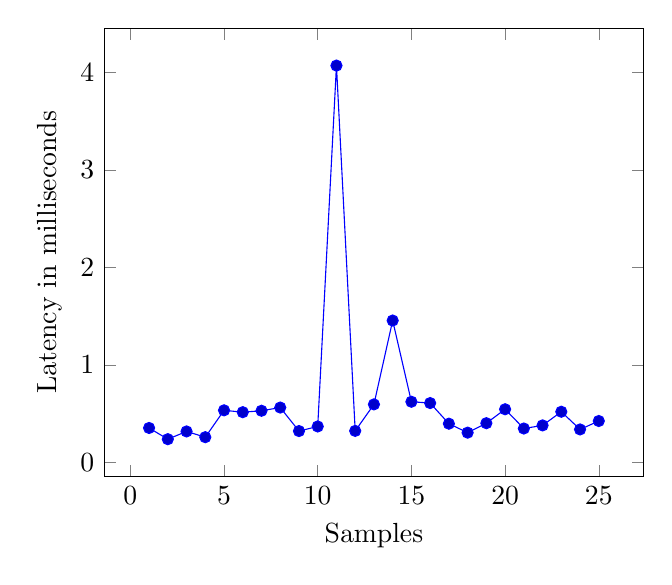
\begin{tikzpicture}
        \begin{axis}[
            xlabel=Samples,
            ylabel=Latency in milliseconds]
            \addplot coordinates {(1,0.352) (2,0.237) (3,0.3165) (4,0.2575) (5,0.533) (6,0.514) (7,0.5285) (8,0.5615) (9,0.3205) (10,0.3675) (11,4.069) (12,0.322) (13,0.594) (14,1.454) (15,0.621) (16,0.6075) (17,0.396) (18,0.304) (19,0.401) (20,0.544) (21,0.3465) (22,0.3785) (23,0.5185) (24,0.337) (25,0.4235) };
        \end{axis}
    \end{tikzpicture}
    \caption{Base-line Cisco Switch: Latency test (One way)}
    \label{CiscoLat}
\end{figure}

